\section*{الف}
ابتدا راسی دلخواه انتخاب می‌کنیم. دورترین راس از‌ آن را پیدا می‌کنیم 
(راس الف)
و سپس دورترین راس از راس پیداشده را پیدا می‌کنیم 
(راس ب). 
مسیر از الف به ب همان طولانی‌ترین مسیر است.

\paragraph{دورترین راس از راس دلخواه}
برای پیدا کردن دور ترین راس از راس دلخواه‌ a به شکل زیر عمل می‌کنیم:
از الگوریتم bfs استفاده می‌کنیم. به این شکل که در هر فراخوانی بازگشتی آن فاصله راس (عمق در درخت پیمایش) را یکی افزایش می‌دهیم. با دیدن راس ها٫ راس با بیشترین فاصله (عمق درخت) و فاصله آن را در دو متغیر global نگهداری و هربار به روزرسانی می‌کنیم. در پایان الگوریتم دورترین راس و فاصله آن را داریم.

\paragraph{
درستی الگوریتم دورترین مسیر
}

\paragraph{
چاپ طولانی‌ترین مسیر
}
حال که راس آغازین و پایانی و طول طولانی‌ترین مسیر را داریم به شکل زیر عمل 
می‌کنیم:

به الگوریتم dfs رفتار جدید اضافه می‌کنیم. یک متغیر گلوبال flag که به طور پیش فرض خاموش است و این به معنی است که الگوریتم dfs به شکل همیشگی رفتار می‌کند. در صورتی که راسی که آن را می‌بنیم همان راس پایانی باشد٫  flag را روشن می‌کنیم و این به این معنی است که الگوریتم دیگر همسایه‌ها را نگاه نمی‌کند و بازگشت به عقب می‌کند و با هر بازگشت آن‌چه در روی آن بازگشتی زده بود را وارد یک استک می‌کند. 
حال اعضای این استک را می‌توانیم پرینت کنیم.

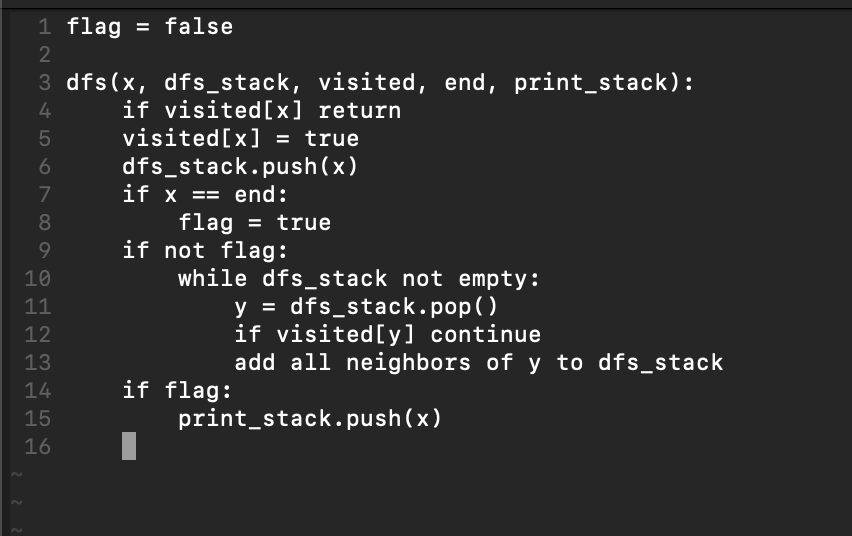
\includegraphics{5-1}

\paragraph{تحلیل مرتبه زمانی}
مرتبه زمان الگوریتم برابر است با چند عمل

\section*{ب}

طول گشت برابر با تعداد دفعاتی است که از یال‌ها عبور می‌کند پس برای کم کردن طول گشت باید یال‌های عبوری را کمینه کنیم. استدلال می‌کنیم که چون همه رئوس باید دیده شود پس گراف تشکیل شده از گشت همبند باید باشد. از طرفی وجود دور در آن غیر بهینه است. چرا که می توانیم به جای عبور از دور و بازگشت به یک راس٫ همان وقتی که در آن هستیم هرکاری که نیاز است بکنیم. پس گراف شبیه به درخت داریم (که البته از بعضی یال‌های آن‌ چند بار عبور کردیم)
.

طول واقعی گشت به شکل زیر خواهد بود:

یک مسیر اصلی داریم که از آن وارد شاخه‌های مختلف می‌شویم و دوباره به آن بر می‌گردیم و مسیر را ادامه می‌دهیم (تا به شاخه‌های دیگر سر بزنیم).

به عبارتی درخت را می‌توان به شکل یک مسیر اصلی (بدنه‌) دید که از بعضی رئوس می‌توان وارد شاخه‌ها شد. 

با این حساب طول گشت برابر با طول مسیر اصلی به علاوه دوبرابر طول مسیرهای فرعی خواهد بود.  و برای کمینه کردن این مقدار کافی است طولانی‌ترین مسیر در این درخت را به عنوان مسیر اصلی انتخاب کنیم. 
اگر تعداد کل یال‌ها m باشد و طولانی ترین مسیر طول x
داشته باشد خواهیم داشت:

\begin{equation*}
	\min y = x + 2*(m-x)
\end{equation*}

